%%%%%%%%%%%%%%%%%%%%%%%%%%%%%%%%%%%%%%%%%
% Journal Article
% LaTeX Template
% Version 1.3 (9/9/13)
%
% This template has been downloaded from:
% http://www.LaTeXTemplates.com
%
% Original author:
% Frits Wenneker (http://www.howtotex.com)
%
% License:
% CC BY-NC-SA 3.0 (http://creativecommons.org/licenses/by-nc-sa/3.0/)
%
%%%%%%%%%%%%%%%%%%%%%%%%%%%%%%%%%%%%%%%%%

%----------------------------------------------------------------------------------------
%	PACKAGES AND OTHER DOCUMENT CONFIGURATIONS
%----------------------------------------------------------------------------------------

%\documentclass[twoside]{article}
\documentclass{article}

\usepackage{lipsum} % Package to generate dummy text throughout this template
\usepackage{url} 

\usepackage[sc]{mathpazo} % Use the Palatino font
\usepackage[T1]{fontenc} % Use 8-bit encoding that has 256 glyphs
\linespread{1.05} % Line spacing - Palatino needs more space between lines
\usepackage{microtype} % Slightly tweak font spacing for aesthetics

\usepackage[hmarginratio=1:1,top=32mm]{geometry} % Document margins
%\usepackage{multicol} % Used for the two-column layout of the document
\usepackage[hang, small,labelfont=bf,up,textfont=it,up]{caption} % Custom captions under/above floats in tables or figures
\usepackage{booktabs} % Horizontal rules in tables
\usepackage{float} % Required for tables and figures in the multi-column environment - they need to be placed in specific locations with the [H] (e.g. \begin{table}[H])
\usepackage[hidelinks]{hyperref} % For hyperlinks in the PDF
\usepackage{amsmath}
\usepackage{graphicx}

\usepackage{lettrine} % The lettrine is the first enlarged letter at the beginning of the text
\usepackage{paralist} % Used for the compactitem environment which makes bullet points with less space between them

\usepackage{abstract} % Allows abstract customization
\renewcommand{\abstractnamefont}{\normalfont\bfseries} % Set the "Abstract" text to bold
\renewcommand{\abstracttextfont}{\normalfont\small\itshape} % Set the abstract itself to small italic text

\usepackage{titlesec} % Allows customization of titles
%\renewcommand\thesection{\Roman{section}} % Roman numerals for the sections
%\renewcommand\thesubsection{\Roman{subsection}} % Roman numerals for subsections
\titleformat{\section}[block]{\large\scshape\centering}{\thesection.}{1em}{} % Change the look of the section titles
\titleformat{\subsection}[block]{\large}{\thesubsection.}{1em}{} % Change the look of the section titles

\usepackage{fancyhdr} % Headers and footers
\pagestyle{fancy} % All pages have headers and footers
\fancyhead{} % Blank out the default header
\fancyfoot{} % Blank out the default footer
%\fancyhead[C]{Running title $\bullet$ November 2012 $\bullet$ Vol. XXI, No. 1} % Custom header text
\fancyfoot[RO,LE]{\thepage} % Custom footer text

\providecommand{\keywords}[1]
{
  \small	
  \textbf{\textit{Keywords---}} #1
}

%----------------------------------------------------------------------------------------
%	TITLE SECTION
%----------------------------------------------------------------------------------------

\title{\vspace{-15mm}\fontsize{24pt}{10pt}\selectfont\textbf{Statistical simulations for measuring operational risks}} % Article title


\usepackage[english]{babel}

\author{
\large
\textsc{Edvard Špaček} \\
\normalsize Prognostickýk klub ČMA \\ % Your institution
\normalsize \href{mailto:edvard.spacek@gmail.com}{edvard.spacek@gmail.com} % Your email addres
\and
\large
\textsc{Jiří Špaček} \\
\normalsize CTU in Prague \\ % Your institution
\normalsize \href{mailto:jiri.spacek@fit.cvut.cz}{jiri.spacek@fit.cvut.cz} % Your email address
\and
\vspace{-5mm}
}
\date{}

%----------------------------------------------------------------------------------------

\begin{document}

\maketitle % Insert title

\thispagestyle{fancy} % All pages have headers and footers



%----------------------------------------------------------------------------------------
%	ARTICLE CONTENTS
%----------------------------------------------------------------------------------------

%\begin{multicols}{2} % Two-column layout throughout the main article text



%----------------------------------------------------------------------------------------
%	ABSTRACT
%----------------------------------------------------------------------------------------

\begin{abstract}

\noindent \emph{Under Pillar 1, Basel II} distinguishes three main risks - market, credit and operational risk. In all cases, it is possible to determine the capital requirement using the basic method, which consists of multiplying the size of the exposure by a predefined coefficient. At the same time, a more advanced approach is allowed for all categories, subject to regulatory approval. The capital requirement may be calculated on the basis of the VaR (ValueAtRisk) method.

In the case of the advanced approach for \emph{operational risk} (the objective of this study), only basic qualitative and quantitative requirements are defined and it is the bank's responsibility to use appropriate methods to estimate the required amount of capital.

\end{abstract}



\keywords{Operational risk, loss distribution, loss frequency, loss severity, composite distribution, AMA methods, LDA approaches, IMA methods, Monte Carlo methods, MILDA\_E calculator, Excel simulation add-ins}


\newpage

%------------------------------------------------

\section{Solution Objectives}

\lettrine[nindent=0em,lines=3]{S} tatistical simulation solutions for finding a composite distribution of losses (magnitudes and frequencies), in \textbf{operational risk} of banks/companies, application of LDA methods (Loss Distrib. Approaches), implementation of MC simulations, including \textbf{program solution} (custom model \textbf{MILDA\_E})


\subsection{Operational risk definition and basic requirements for the advanced approach}

Operational risk is defined in the CRD (Capital Risk Directive) as the risk of loss arising from deficiencies or failures in internal processes, people and systems or from external events and also includes legal risk. Quantitative requirements include the requirement to achieve a confidence level of 99.9\%. The capital requirement must include both expected and unexpected losses. The operational risk measurement system (and the determination of risk-based capital) must take into account the \emph{tails} of the loss distribution.

The operational risk measurement system must take into account the four elements of the advanced approach - internal and external data, scenario analysis, business environment factors and internal control factors. The different elements may be taken into account in different ways and at different stages of modelling, and the CRD leaves a large degree of discretion to individual banks in this area. A bank may still take into account the effect of insurance before the final capital requirement is determined. This is what the definition says.




\section{Simulation model for calculation of composite frequency distribution and loss significance}

\textbf{This paper will focus on the Loss Distribution Approach (LDA), which is based on statistical methods applied to internal/external ordinary loss data (with a moderate tail of the distribution). The objective was to demonstrate the effectiveness of simple means in calculating risk-based capital using an Excel spreadsheet and relevant simulation add-ins.}

Furthermore, the existing software for the implementation of Monte Carlo, as well as other methods suitable for risk calculations, was mapped.
As part of the solution, the described problem and the solution using the Internal Measurement Approach (IMA) method, assuming a normal distribution of loss severity and a Poisson distribution of loss frequency, were used.

As the \textbf{main problem} in the task of implementing MC simulations, finding a \emph{composite distribution} of the total losses by LDA was analyzed. It is necessary to perform statistical simulations of the distribution of total loss values based on simulations of frequency distributions (\emph{Poisson, alternatively Binomial}) and the distribution of individual loss values (\emph{lognormal}). \emph{Alternatively}, more sophisticated analytical procedures are available to calculate the composite distribution of total losses (see Panjer et al, 1998 \cite{loss}). The main output in this section is the implementation of the MC method algorithm by simulations on the LDA solution in a concrete implementation in the \textbf{MILDA\_E model}. This assumes that verified parameters of the input distributions are available (this step is not included).

\subsection{SW dependencies}

\begin{compactitem}
\item Windows 7, Excel 2003 and lower (higher versions not tested), Jensen simulation libraries (available on the web)
\item libraries ran\_var, simulation, simtools, installed as Excel add-ins
\item Excel functions POISINV, LNORMINV (check)
\item our application MILDA\_E
Note: If the Visual Basic (Excel) module reports an error, it is usually because the Jensen libraries are not compatible with one of the other system components. Since the libraries are unavailable, there is no remedy other than to swap versions of the system (preferably in a virtual machine, which does not interfere with the existing configuration) and Excel.

\end{compactitem}

A simplified solution was described using the Internal Measurement Approach (IMA), assuming a normal distribution of loss severity and a Poisson distribution of loss frequency. The numerical results of the IMA method can be used for a rough comparison with the outputs of MC simulations.

%------------------------------------------------

\section{Solution of the LDA problem (with comparative calculations using IMA) and description of the presented calculation program MILDA\_E}

\subsection{Overview of AMA methods investigated in the task}

\begin{compactitem}
\item IMA (Internal Measurement Approach)				(1)
\item LDA (Loss Distribution Approach)				(2)
\end{compactitem}

Methods of type (1), (2) are statistical in nature. This approach monitors the occurrence of loss phenomena and their magnitude and measures them with statistical characteristics. As a result, the amount of capital contribution is derived from these values. The factor of time is not taken into account, the occurrence and magnitude of losses have stable probability distributions, unchanging over the period of the year under consideration.


\subsection{Business lines and risk types in terms of statistical approach, aggregation of sub-capital requirements}

In order to achieve greater homogeneity of processing, the entire scope of the OR in the bank is divided into a matrix consisting of 8 business lines and 7 risk types. This also applies to the statistical description applied by methods (1), (2). It is necessary to subject the individual fields of the matrix to partial \emph{statistical} procedures. The LDA and IMA methods respond to this requirement by calculating the partial loss distributions. For the smooth application of these methods, it is necessary that the loss values and their frequencies come from a statistically homogeneous source. It is not desirable that the loss distributions (within a matrix) are a mixture of several types of distributions. Also, the corresponding sub-capital requirements need to be aggregated into an aggregate.

\subsection{Brief characteristics of statistical AMA methods used}

For these methods, \emph{empirically} measured loss data with a minimum 3 year history is required. These data need to be transformed into the shapes of loss probability distributions. They are further used for the purpose of \emph{validating} certain theoretical probability distributions and determining their \emph{parameters}. From these theoretical distributions, the \emph{statistical characteristics of interest} are calculated using analytically derived relations or simulation techniques. Validation is performed by testing statistical \emph{hypotheses} that the observed data confirm the validity of the specified type of distribution at a given level of significance. To determine the shapes and parameters of the distribution, a longer interval of observation of the loss data is required so that the resulting estimates of the parameters of the distribution of the loss phenomena are based on sufficiently numerous observations.

For processing, two statistical features are taken into account - the \emph{occurrence} of loss phenomena and their \emph{significance} (value). Both are subject to certain probability distributions that need to be estimated from the data. These distributions are different for the two aspects of the loss data and differ in the magnitude of the parameters and between the elements of the matrix (intercepts B/L $\times$ E/T). In addition, a monitoring horizon of 1 year is essential.


\textbf{(1) IMA} is based on the following inputs:

\begin{compactitem}
    \item Total number of potential loss phenomena
    \item Probability of a loss event within this set (frequency of occurrence)
    \item Mean and standard deviation of the loss (magnitude of the loss)
\end{compactitem}

The IMA is characterised by setting the unexpected loss as a multiple of the expected loss. The \emph{Capital} requirement is given by the unexpected loss. It is derived as the product of:

\begin{compactitem}
    \item the gamma coefficient $\gamma$,
    \item the indicator \emph{exposure} to risk (potential loss incidence),
    \item the \emph{probability} of a loss event (in terms of frequency), and
    \item \emph{average loss}, (in terms of severity)
\end{compactitem}

at a given confirmation margin (e.g. set for banks at 99.9 \%).

Two types of distributions appear in the formula, for the frequency of loss events and the magnitude of losses. Analytically, the binomial (for smaller frequency of occurrence) and Poisson distributions are used, respectively.  For the magnitude of losses, the normal distribution is used.

\textbf{(2) LDA} type methods are based on direct measurement of unexpected loss as a characteristic of \emph{composite frequency distribution} and loss severity. The \emph{lognormal} distribution is used as a type of distribution of loss values. The frequencies of occurrence of loss phenomena are again binomial or Poisson. The unexpected loss is quantified as 99.9 \% quantile of the composite probability distribution minus the expected loss. The capital requirement is therefore calculated from the characteristics of the composite distribution. When applying the LDA procedure, the basic problem is the calculation of the composite distribution. It introduces the assumption of the size of the unexpected loss as a multiple of the expected loss.

The application of both procedures results in a capital requirement for operational risk. This requirement is given by the sum of the requirements in each risk line and risk type, assuming statistical independence of the occurrence of losses and their values for each field of the matrix. Theoretically (assuming independence), this leads to the so-called \emph{convolution} of the distribution, to the calculation of an aggregate distribution under uncorrelated losses.

Briefly summarized:
\begin{compactitem}
    \item IMA is technically simpler than LDA, where a composite loss distribution is assumed
    \item The LDA approach is probably preferable, IMA is simpler, the difference is in the combination of distribution types
    \item LDA leads to aggregation of distributions, IMA introduces a simplifying assumption and does not go into detail in the statistical description
    \item The input to LDA is the frequency distribution of loss phenomena (usually Poisson) and the distribution of losses (lognormal). The result is a composite true distribution of loss values weighted by their incidence.
\end{compactitem}


\subsection{Brief IMA calculation algorithm}

This is based on the number of $N$ events potentially burdened with op-risk in the annual horizon. Further, the \emph{probability} of a loss event $p$ from these $N$ possible events.
The basis is an estimate of the \emph{expected} loss $N * p * \mu_L$. To do this, we need to estimate the average loss from one event $\mu_L$. This characteristic is calculated from two sources, the distribution:

\begin{itemize}
  \item A) Frequencies of losses (binomial distribution); parameters $N$, $p$
  \item B) Loss severities (normal distribution); parameters $\mu_L$, $\sigma_L^2$ (mean value, variance)
\end{itemize}

Calculations of the distributions $A$ and $B$ and their characteristics yield the magnitudes of $\gamma$ from the value of the coefficient $k$. The IMA is characterized by the fixed size of the difference between the \emph{expected} (the mean of the distribution) and the \emph{unexpected} loss (the tail of the distribution given by 99.9% credibility).

In theory, formulas are derived:

\begin{equation}
  \gamma = k * \frac{\sqrt{1 + (\frac{\sigma_L}{\mu_L})^2}}{\sqrt{N * p}}
\end{equation}

where $k = \frac{(\alpha \textrm{ percentile of distrib.  } B - N * p)}{\sigma_L}$

A simpler form of the formula is (with unknown variance $\sigma_L$):

\begin{equation}
  \begin{aligned}
  \gamma &= \frac{k}{\sqrt{N * p}} \\
       k &= k * \mu_L \sqrt{N * p}
  \end{aligned}
\end{equation}

The alternative distribution to $A$ (frequency) is Poisson, to $B$ (loss) lognormal.

\textbf{Capital requirement calculation}

The OR capital requirement is determined by the unexpected loss, the expected loss is covered by reserves that can be set aside a priori. This is derived using the coefficient $\gamma$, an indicator of the exposure $EI$ to risk, e.g. loss phenomenon $PE$ and the average loss $LGE$, $I$, $J$ denotes the line/type, $K$ denotes the capital requirement.

\begin{equation}
  K_{i,j} = \gamma_{i,j} * EI_{i,j} * PE_{i,j} * LGE_{i,j} = \gamma_{i,j} * EL_{i,j}
\end{equation}


The calculation according to the IMA algorithm is taken as a guideline for the purpose of comparing the results with the LDA method, whose results are taken as a reference.

\subsection{Brief calculation algorithm according to LDA}

The goal is to create a model for aggregate losses - to determine the probability distribution for the total loss.

\emph{The total loss} $S$ is defined as the sum of:

\begin{equation}
  S = X_1+…+X_N (N = 0,1,2 \ldots)
\end{equation}

random number $N$ of individual losses ($X_1 \ldots X_N$). The assumption of independence and equal distribution of $X_i$ is introduced. Also, $N$ and $X_i$ are independent. That is:

\begin{compactitem}
\item Assuming $N = n$, the random variables $X_1 \ldots X_n$ are independent and equally distributed
\item The distribution of $N$ does not depend on the values of $X_1,X_2 \ldots$.
\end{compactitem}

The calculation problem focuses on:
\begin{compactitem}
\item Estimation of probability distribution for $N$ based on random sampling
\item Estimation of Probability distribution for $X_j$ based on random sampling
\item Using these distributions, construct the distribution of random variable $S$
\item The distribution (4.3) is called the composite distribution.
\end{compactitem}


\begin{figure}[H]
  \caption{LDA characteristics, see article EVT-box}
  \centering
    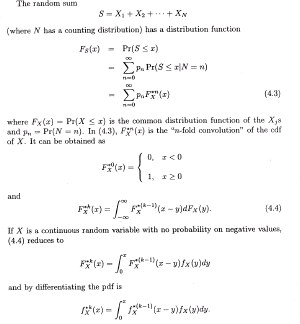
\includegraphics[width=0.6\textwidth]{ldachar}
\end{figure}


%% The random sum

%% \begin{equation}
%%   S = X_1 + X_2 + \cdots + X_N
%% \end{equation}

%% (where $N$ has a counting distribution) has a distribution function

%% \begin{equation}
%%   \begin{aligned}
%% F_s(x) &= P_x(S \leq x) \\
%%       &= \sum_{n=0}^{\infty}p_nP_x(S \leq x | N = n) \\
%%       &= \sum_{n=0}^{\infty}p_nF_X^n\{x\}
%%       \end{aligned}
%% \end{equation}

%% where $F_X(x) = P_x\{X \teq x\}$ is the common distribution function of the $X_j$ and $p_n = Px\{N = n\}$. In (d.3), $F_x^n\{x\}$ is the n-fold convolution of the cdf of $X$. It can be obtained as

%% smth

%% and

%% F_X^{\lambda}(X) = \int_{-\infty}^{\infty}


\subsection{Analytical methods for calculating the composite distribution.}

Under certain circumstances, the normal or lognormal distribution can be a good approximation of the distribution. S. This concerns the limiting values of the parameters of the Poisson distribution.

Obviously, the direct calculation according to (4.3) is not straightforward. An \emph{approximation} of the distribution using the known moments of the distribution is offered. There are significant drawbacks to this solution; a satisfactory degree of agreement of the approximation with the true distribution is not known.

The \emph{direct} convolution method (4.4) leads to numerical integration, which is a computationally demanding task. The complexity is somewhat reduced by replacing the continuous distribution of X by a discrete one, yet this route remains difficult.

Another \emph{recursive} method invents a reduction in the number of computational steps according to the above direct computation method, but it depends on certain types of distributions. Nevertheless, it remains a suitable method for verifying results from multiple sources.

The last method uses the \emph{inversion} of the characteristic function and uses the appropriate software. This method also deserves attention as a promising but specialized one. Both recursion and inversion are based on the assumptions of independence and equal distribution. For the approximative method, histogram approximation is required. The assumption of equal distribution over a long time interval does not seem to be completely realistic. The problem is that a higher incidence of loss phenomena leads to corrective measures that reduce their incidence and thus modify the original loss distribution, which then follows a different law.


\subsection{Simulation method}

This process can be characterized as follows:


\begin{itemize}
  \item Build a mode for $S$ which depends on random variable $X, Y, Z\ldots$
  \item For $i = 1,\ldots,n$ generate pseudorandom variables $x_i,y_i,z_i\ldots$ and then compute $s_i$ using the model from step 1
  \item The cdf of $S$ may be appropriated by $F_S\{s\}$, the empirical cdf based on the pseudorandom sample $s_1,\ldots,s_n$.
\end{itemize}

The goal is to determine an empirical distribution function based on a sequence of (pseudo) random numbers $s_1, \ldots s_n$. The question is how large n to choose. Clearly, as the number of values increases, a correct estimate can be achieved with an increased degree of precision.  It is not a problem to shift it effectively to the order of $10^4$. We take the empirical values of their estimates (e.g. sample means, standard deviations, quantiles, etc.) as the characteristics of the observed distribution we are looking for. We are confident that with a sufficiently large number of observations, these characteristics can be identified (according to the law of large numbers), with a high degree of precision, with the sought-after unknown values of the underlying distribution.

This is also useful for our case of finding the aggregate loss distribution. Therefore, this method of calculation, which is an alternative to analytical procedures, is advantageous. Algorithmically, it is simple but requires a large number of computations, which is not so much of a problem.

The process of aggregating the loss distributions within the matrix can be shown \emph{schematically}:

\begin{figure}[H]
  \caption{}
  \centering
    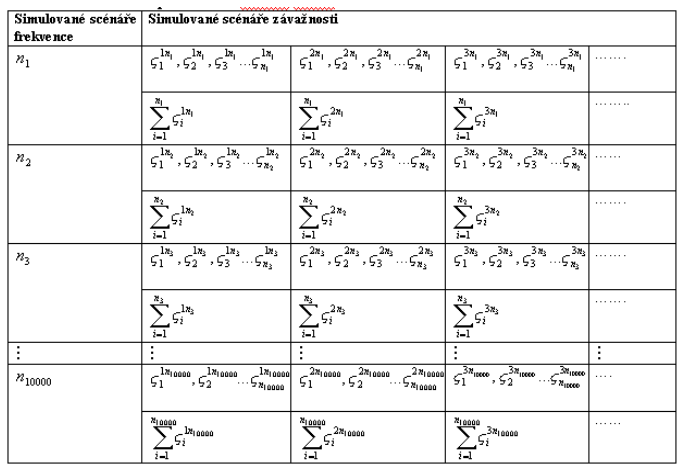
\includegraphics[width=0.75\textwidth]{simul_scenare}
\end{figure}


A simulation analogy with a roll of two dice:

\begin{figure}[H]
  \caption{}
  \centering
    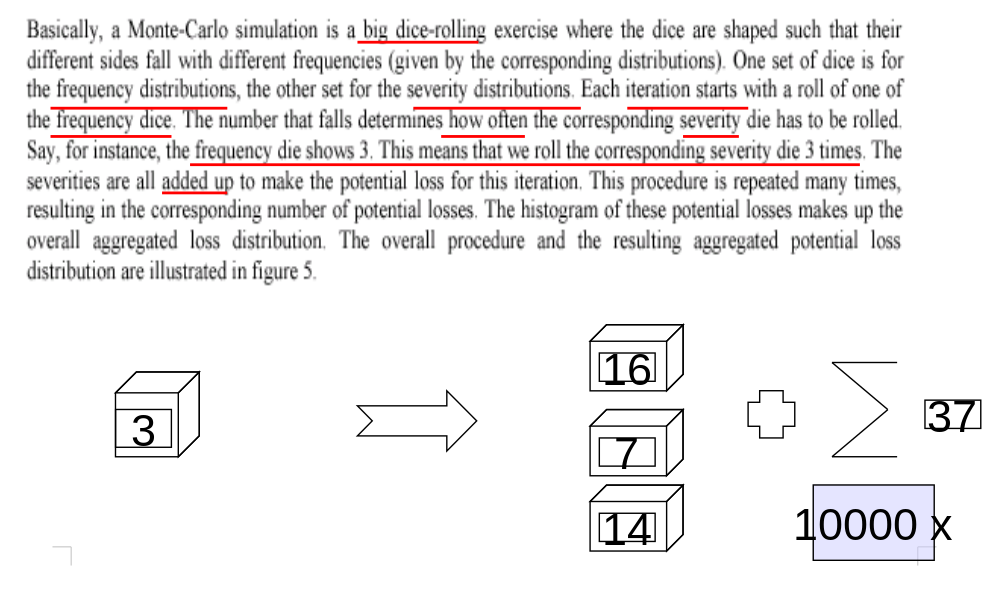
\includegraphics[width=0.75\textwidth]{kostky}
\end{figure}


\begin{figure}[H]
  \caption{Expected and unexpected losses within the distribution}
  \centering
    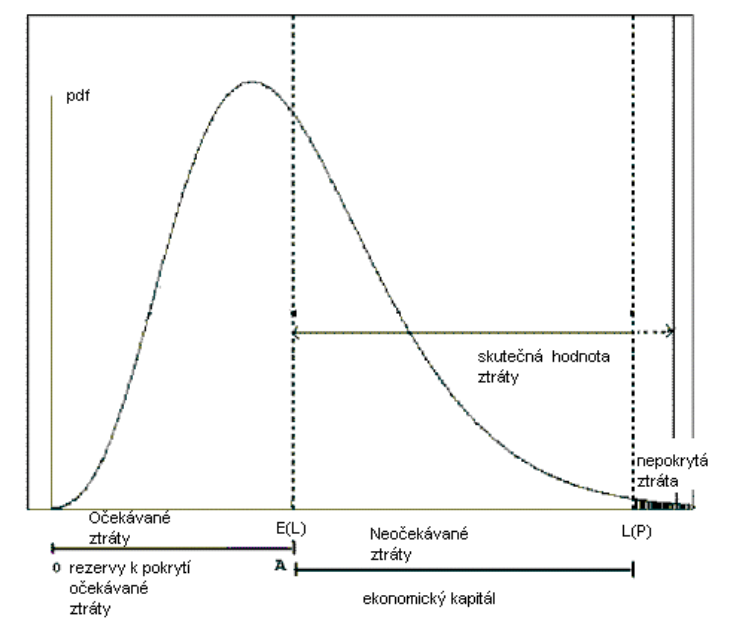
\includegraphics[width=0.75\textwidth]{ztraty}
\end{figure}


\begin{figure}[H]
  \caption{Simulation calculation scheme for business lines, risk types}
  \centering
    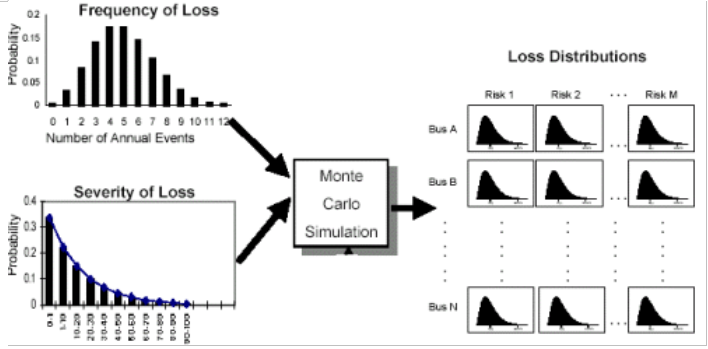
\includegraphics[width=0.75\textwidth]{schema}
\end{figure}



%------------------------------------------------

\section{Implementation of MC simulations}


\subsection{Excel program „MILDA\_E – Malý Ima LDA kalkulátor (Excel)“}

The initial software solution for simulation calculations is prepared in Excel. The calculation is performed in six sheets. The aim is to convert the above algorithm into a formal program form suitable for the interactive calculation of the above characteristics, including the capital requirement. The calculation is performed in parallel for two types of distributions, Binomial and Poisson on the quotient side, of lognormal weight. The analytical figures are accompanied by a graphical representation with automatic recalculation of the shape of the distribution and its characteristics when the input data are changed.

List and functionality of worksheets:
\begin{compactitem}

\item \textbf{Výběr}: shows list BL/ET (matrix k8x7 for banks), after
  the user makes a selection, it moves to the sheet:
\item \textbf{Vstupy\_a\_Výstupy}: for the selected BL/ET combination, the inputs and the calculation of the output values are introduced
\emph{vstupy} - the number of loss phenomena $N$, the probability of loss phenomena $p$, the coefficient $\lambda$ of the Poisson distribution, the average loss and variance of the loss distribution, the confidence limit $\alpha$,
\emph{výstupy} IMA - capital contribution of type \textbf{a} (with knowledge of loss severity variance) and \textbf{b} (without knowledge of loss severity variance), expected total loss
  
Sheet contains an LDA softkey that moves the calculation to the next \textbf{simulation phase}.
\item \textbf{Poisson\_distr.}: contains calculations based on the Binomial distribution
\item \textbf{Poisson\_distr.}: contains calculations based on the Poisson distribution
The last two sheets are complemented by the Normal distribution of loss severities.
\item \textbf{Simulace}: It is a sheet in which the computations of the composite distribution are performed. The empirical distributions of frequencies and loss magnitudes are generated (using pseudo-random numbers) and displayed. The computation problem focuses on generating random upper bounds for the summed $s_n$ values. An algorithm has been prepared that converts the random numbers generated from the Poisson distribution of occurrences into the computation of random upper bounds for the summation cells. These summation values (in aggregate) produce an empirical distribution of aggregate losses. A histogram of this distribution is calculated using the appropriate Excel function. In addition, the mean, standard deviation, 0,999 quantile and, derivatively, the capital contribution for operational risk coverage are calculated.
\textbf{Simulace (2)}: is a sheet in which the calculated values of the characteristics of the composite distribution are displayed

\end{compactitem}

\subsection{Program characteristics}

The calculation uses Excel's statistical and search functions, including Visual Basic macros within Excel. The calculation is supported by a number of simulation libraries to generate pseudo-weighted numbers from prescribed distributions. These libraries are installed as Excel add-ins.

Can be found at \cite{addins}

The basic element permeating the calculations is \emph{SIMULATION TABLE}, in a selected range, tabulates outputs from repeated recalculations of a MC simulation model. The outputs to be tabulated should be in the top row of the selected range, but the top-left cell of this selected range should be unused. Recalculated values of the simulation outputs will fill the lower rows of the selected range, with each row containing the output values from an independent recalculation of the simulation model. The left column of the selected range is used for a percentile index, which can be useful for making cumulative-distribution charts after the output data is sorted (but the Simulation Table procedure itself does not sort the output data).

It is not a limitation (due to the use of other analytic functions) to calculate the Binomial distribution for a large value of the product $N * p$, also a Poisson distribution. even for high $\lambda$.  For $\mu, \sigma$,  no restriction on values is required. For this calculation, the capital ratio is set as the target, then the parameters $N$, $p$, $\lambda$, $\mu_l$, $\sigma_L^2$ as influencing parameters. It also allows to determine how sensitive the change in the capital requirement is to the input values.


\subsection{Graphic design of input/output sheets}

\begin{figure}[H]
  \caption{Selection (business lines, risk types)}
  \centering
    
\includegraphics[width=0.75\textwidth]{matice}
\end{figure}


\begin{figure}[H]
    \caption{Inputs and outputs (parameters of loss distributions)}
  \centering
    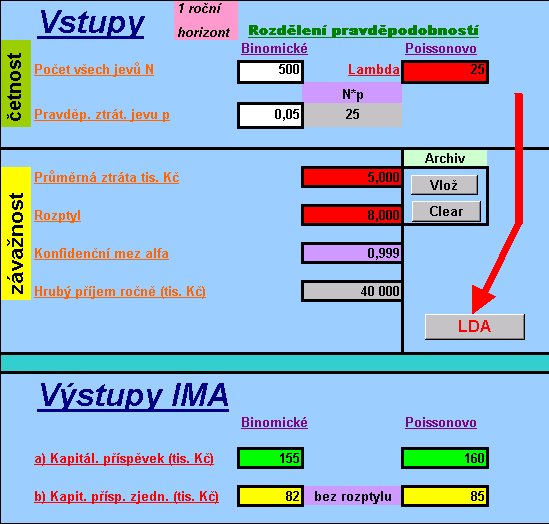
\includegraphics[width=0.75\textwidth]{vstup}

\end{figure}

\begin{figure}[H]
  \caption{Simulation of frequency distribution and loss severity (distribution aggregation)}
  \centering
    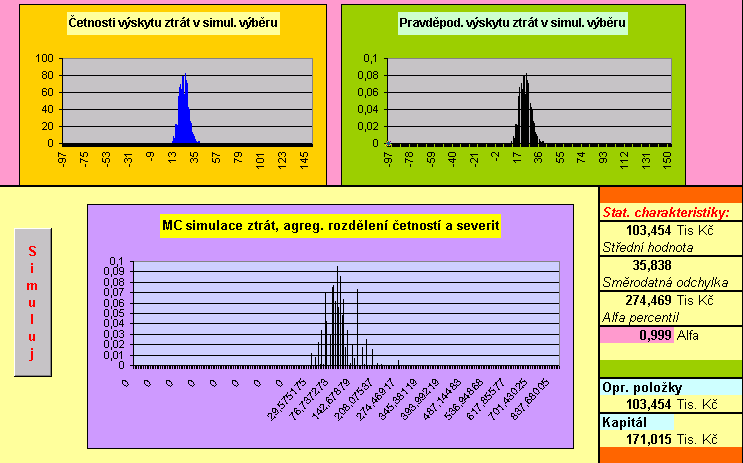
\includegraphics[width=0.75\textwidth]{simuluj}
\end{figure}

\begin{figure}[H]
  \caption{Calculation detail for business line 3 and type 2}
  \centering
    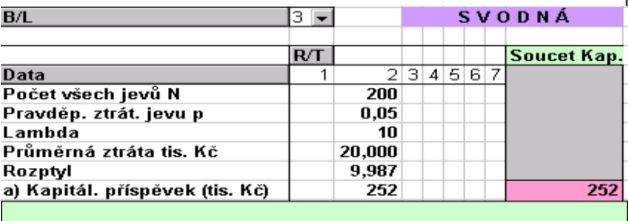
\includegraphics[width=0.75\textwidth]{tabulka}
\end{figure}

This table provides information on the amount of capital per line for all types and the distribution parameters used. If we select "ALL" as the line, then only the capital row is meaningful and we get the sum for all lines/types and the total capital amount.


\subsection{Further development of the program}

Further use is determined by the possibilities of Excel for a high number of simulated values from the densities of Binomial and Poisson distributions, 1000 simulations are performed in the program. For refinement purposes, the number of simulations should be increased to 5 to 10 thousand. A useful extension would be a sensitivity analysis, back-calculating the influencing values of the distribution parameters from the prescribed \emph{target value} of the risk capital contribution. This would make it possible to see what loss distribution parameters lead to the appropriate level of a given capital requirement. This is also relevant when knowledge of the distribution parameters is incomplete and we cannot rely on reliable estimates. This functionality is commonly obtained by using Excel's "solver" function, which allows the equation to be solved backwards for one parameter at a time. However, such a procedure cannot logically be applied to the value obtained by the simulations. It is necessary to perform multiple simulations with impact tracking.

The introduction of AMA methods and their appropriate use can lead to a reduction in the capital requirement by influencing the loss process towards a reduction in loss incidence and severity.

\section{Brief characteristics of Monte Carlo simulation methods}

Numerical methods, which are known as Monte Carlo methods, can be described as statistical simulation methods, where statistical simulation is defined as a method using sequences of random numbers to perform simulations.

Statistical simulation methods can be compared with conventional numerical methods. In many Monte Carlo applications, the procedure is simulated directly. The only requirement is that the system is described by a \emph{probability density function}. If the probability density is known, the Monte Carlo simulation can proceed by randomly selecting from the population given by this density. Then an order of magnitude of simulations are performed and the desired result can be taken as the average of a number of observations.

\subsection{Main components of the Monte Carlo algorithm}

The components of the Monte Carlo simulation are as follows:

\begin{compactitem}

\item probability distribution functions (densities) - the system must be described by a set of densities
\item Random number generator (source)
\item Selection rule - a rule for selecting from a specified distributino
\item Error estimation - estimate of statistical error (variance)
\item Variance reduction techniques - methods for reducing variance in the estimated solution

\end{compactitem}

The goal of the Monte Carlo method is to simulate a given system using samples from a population with these densities.

\subsection{Conclusions}

The problem statement is based on the needs of risk quantification and management, in particular the determination of risk capital. A statistical approach is applied to advanced operational risk measurement methods, which is the basis of Advanced Measurement Approach (AMA) methods. This statistical modelling approach results in risk concepts and methods being introduced in a methodologically consistent manner. Statistical methods have a useful place in the determination of ValueAtRisk (here OpVar) and the determination of the capital contribution to cover unexpected losses. Their use leads to advanced techniques, including \emph{Monte Carlo simulations}. These techniques have proven to be viable in implementations, simplifying the finding of solutions, shifting the focus of the problem to the computer and bypassing difficult analytical formulas. The results of simulations should be viewed in the same way as any empirical data. The question of the plausibility of the characteristics obtained by MC simulations in terms of sample size and stability of the estimates is logically raised. A large number of simulations (of the order of $10^4$) need to be performed.


\nocite{*} % include all references without citations

\bibliographystyle{plain} % We choose the "plain" reference style
\bibliography{refs} % Entries are in the refs.bib file

%Operational Risk: Practical Approaches to Implementation, edited by Ellen Davis, RiskBooks, 2005
%Loss Models from data to decisions, S.A. Klugman, H.H. Panjer, G.E. Willmot; John Wiley & Sons, 1998
%Quantifying Operational Risks within Banks according to Basel II, M.R.A. Akker, TUDelft, 2004
%https://real-statistics.com/

%----------------------------------------------------------------------------------------

%\end{multicols}

\end{document}
